% =====================================================================
%  O termo não conservativo e a dependência do caminho
%  Nota complementar ao minicurso + conferência da Definição 4.2 das notas de rDG do RELAP-7
%  Compilar com lualatex. Figuras: scripts/ (Python 3 + numpy + matplotlib)
% =====================================================================
\documentclass[11pt,a4paper]{article}
\usepackage[margin=2.4cm]{geometry}
\usepackage{fontspec}
\usepackage[brazil]{babel}
\usepackage{amsmath,amssymb,amsthm,mathtools}
\usepackage{booktabs,array}
\usepackage{graphicx}
\usepackage[most]{tcolorbox}
\usepackage{tikz}
\usetikzlibrary{arrows.meta,decorations.pathreplacing,calc}
\usepackage{caption}
\usepackage{enumitem}
\usepackage[hidelinks]{hyperref}

\definecolor{azul}{HTML}{103460}
\definecolor{laranja}{HTML}{ED7D31}
\definecolor{verde}{HTML}{146E46}
\definecolor{vermelho}{HTML}{AA3228}
\definecolor{azulclaro}{HTML}{5B9BD5}

\captionsetup{font=small,labelfont=bf}
\setlist{itemsep=2pt,topsep=4pt}
\AtBeginDocument{\setlength{\abovedisplayskip}{6pt}\setlength{\belowdisplayskip}{6pt}}

\newtcolorbox{intuicao}{enhanced,colback=black!4,colframe=black!25,boxrule=0.5pt,arc=1pt,
  left=6pt,right=6pt,top=4pt,bottom=4pt,before upper={\textbf{Intuição.}\enspace}}
\newtcolorbox{mensagem}{enhanced,colback=laranja!12,colframe=laranja!70,boxrule=0.5pt,arc=1pt,
  left=6pt,right=6pt,top=4pt,bottom=4pt,fontupper=\bfseries}
\newtcolorbox{quadro}[2]{enhanced,colback=#1!4!white,colframe=#1,colbacktitle=#1,coltitle=white,
  fonttitle=\bfseries,title={#2},boxrule=0.5pt,arc=1pt,left=6pt,right=6pt,top=4pt,bottom=4pt}

\theoremstyle{definition}
\newtheorem{definicao}{Definição}[section]
\newtheorem{proposicao}[definicao]{Proposição}
\theoremstyle{remark}
\newtheorem{observacao}[definicao]{Observação}

\newcommand{\pd}[2]{\frac{\partial #1}{\partial #2}}
\newcommand{\dd}{\mathrm{d}}
\newcommand{\Fh}{\widehat F}
\newcommand{\ub}{\bar u}

\begin{document}

\begin{center}
{\LARGE\bfseries O termo não conservativo e a dependência do caminho}\\[6pt]
{\large Explicação passo a passo e conferência da Definição 4.2 das notas de rDG do RELAP-7}\\[6pt]
{\small Nota complementar ao minicurso de métodos numéricos para leis de conservação \quad·\quad Outubro de 2026}
\end{center}

\begin{quadro}{verde}{Resumo}
Um termo não conservativo é o produto de um coeficiente pela derivada de outra grandeza. Onde a solução é suave ele é uma função comum. Num salto vira ``degrau vezes Dirac'', cujo valor depende do que acontece \emph{dentro} do salto: esse ``o que acontece dentro'' é o \textbf{caminho}. A Parte~I explica a ideia com um cálculo de duas linhas, uma figura, uma analogia com o trabalho termodinâmico, um exemplo de engenharia (a expansão brusca num duto) e um experimento numérico. A Parte~II usa essas ideias para conferir a Definição 4.2 das notas. Ela está correta: $D^-_{i+1/2}$, $D^+_{i-1/2}$ e $G_i$ medem pedaços disjuntos do mesmo produto, não há contagem dupla e os três são necessários.
\end{quadro}

\tableofcontents

% =====================================================================
\part*{Parte I --- O termo não conservativo e o caminho}
\addcontentsline{toc}{part}{Parte I --- O termo não conservativo e o caminho}

\section{O que é um termo não conservativo}

\begin{intuicao}
Num duto de seção variável $A(x)$, a parede inclinada empurra o fluido. Numa fatia de comprimento $\dd x$ a força axial vale $p\,\dd A$; na equação do momento ela aparece como $p\,\partial_x A$. Esse termo não é a derivada de grandeza alguma: é o produto de uma grandeza (a pressão) pela derivada de outra (a área). Todo termo não conservativo tem essa forma: um coeficiente vezes a derivada de outra coisa.
\end{intuicao}

Considere sistemas da forma
\begin{equation}\label{eq:sistema}
\pd{U}{t}+\pd{F(U)}{x}+B(U)\,\pd{U}{x}=0 .
\end{equation}
O termo $B(U)\,\partial_x U$ é \emph{conservativo} quando existe uma função $G$ com $B=DG$ (a matriz jacobiana de $G$). Nesse caso $B(U)\,\partial_xU=\partial_x G(U)$ e ele pode ser somado ao fluxo. Caso contrário, é \emph{não conservativo}. Na prática ele aparece como $c(U)\,\partial_x w$, em que $w$ é uma das componentes de $U$. Esse produto só é conservativo quando $c$ depende apenas de $w$, pois então $c(w)\,\partial_xw=\partial_x\mathcal C(w)$ com $\mathcal C'=c$. A Tabela~\ref{tab:exemplos} reúne os casos que nos interessam.

\begin{table}[h]
\centering\small
\caption{Termos não conservativos em modelos usuais: sempre um coeficiente vezes a derivada de outra grandeza.}\label{tab:exemplos}
\begin{tabular}{@{}llll@{}}
\toprule
modelo & termo & coeficiente & derivada de\\
\midrule
duto de seção variável & $p\,\partial_xA$ & pressão & área\\
sete equações (BN) & $p_I\,\partial_x\alpha_k$, $p_Iu_I\,\partial_x\alpha_k$, $u_I\,\partial_x\alpha_1$ & $p_I$, $u_I$ & fração de volume\\
energia interna (RELAP5) & $p\,\partial_xu$ & pressão & velocidade\\
águas rasas com fundo variável & $g\,h\,\partial_xb$ & profundidade & cota do fundo\\
\bottomrule
\end{tabular}
\end{table}

Onde a solução é suave, o produto é uma função comum: multiplica-se o coeficiente pela derivada, ponto a ponto, sem nada a discutir. A dificuldade aparece quando o coeficiente e a grandeza derivada saltam \emph{no mesmo ponto}.

% ---------------------------------------------------------------------
\section{O problema num salto: quanto vale ``degrau vezes Dirac''?}

\begin{intuicao}
Se $u$ e $w$ saltam no mesmo ponto, $\partial_x u$ é uma Dirac e $w$ é um degrau. Perguntar quanto vale $w\,\partial_xu$ é perguntar qual valor de $w$ usar no instante em que $u$ salta: o da esquerda, o da direita ou algo entre eles. A resposta depende de qual das duas grandezas muda primeiro dentro do salto. O modelo sem viscosidade não tem essa informação.
\end{intuicao}

Tome o caso mais simples: $u$ e $w$ passam de $0$ a $1$ em $x=0$. Para dar sentido a $w\,\partial_xu$, troque cada salto por uma rampa de largura $\varepsilon$,
\[
u_\varepsilon(x)=r\Big(\frac{x-a}{\varepsilon}\Big),\qquad w_\varepsilon(x)=r\Big(\frac{x-b}{\varepsilon}\Big),\qquad r(\xi)=\min\big\{\max\{\xi+\tfrac12,\,0\},\,1\big\},
\]
e calcule $I_\varepsilon=\int w_\varepsilon\,\partial_xu_\varepsilon\,\dd x$ (Figura~\ref{fig:degrau}):
\begin{enumerate}[label=(\alph*)]
\item $w$ termina de mudar antes de $u$ começar: durante a rampa de $u$ vale $w=1$, logo $I_\varepsilon=1$;
\item as duas mudam juntas ($a=b$): $I_\varepsilon=\int r\,r'\,\dd\xi=\big[r^2/2\big]=1/2$;
\item $u$ termina de mudar antes de $w$ começar: durante a rampa de $u$ vale $w=0$, logo $I_\varepsilon=0$.
\end{enumerate}
Quando $\varepsilon\to0$, as três regularizações convergem para as \emph{mesmas} funções descontínuas $u$ e $w$. Mesmo assim $I_\varepsilon$ não muda: vale $1$, $1/2$ ou $0$ para todo $\varepsilon$. Com sobreposições parciais das rampas obtém-se qualquer valor entre $0$ e $1$. O limite dos produtos depende de como os produtos foram construídos; o ``produto dos limites'' simplesmente não está definido.

\begin{figure}[h]
\centering
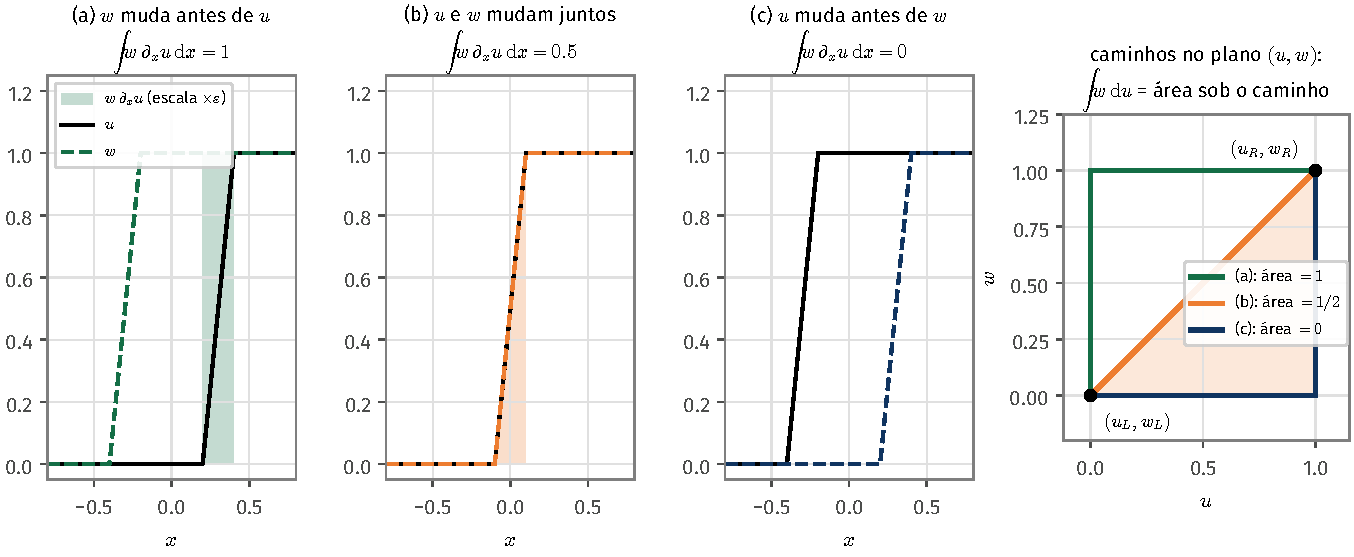
\includegraphics[width=\textwidth]{figs/degrau_dirac.pdf}
\caption{O mesmo salto de $u$ e $w$ (de $0$ a $1$), regularizado de três modos. Em (a), (b) e (c), a área colorida é $w\,\partial_xu$ (multiplicado por $\varepsilon$ para caber no gráfico); a sua integral não depende de $\varepsilon$. À direita, as três regularizações vistas no plano de estados: cada uma é um caminho de $(u_L,w_L)$ a $(u_R,w_R)$ e o valor do produto é a área sob o caminho.}\label{fig:degrau}
\end{figure}

% ---------------------------------------------------------------------
\section{O caminho: a mesma ideia vista no espaço de estados}

\begin{intuicao}
Esqueça a variável $x$ e olhe só para os estados. Quando $x$ atravessa o salto, o par $\big(u(x),w(x)\big)$ desenha uma curva que sai de $(u_L,w_L)$ e chega a $(u_R,w_R)$. Essa curva é o \emph{caminho}. O valor de $\int w\,\partial_xu\,\dd x$ é a área sob ela.
\end{intuicao}

A mudança de variável $x\mapsto\big(u(x),w(x)\big)$ transforma a integral em $x$ numa integral de linha,
\[
\int w\,\pd{u}{x}\,\dd x=\int_\gamma w\,\dd u ,
\]
em que $\gamma$ é a curva percorrida pelos estados. No painel da direita da Figura~\ref{fig:degrau}, os três casos são três curvas com as mesmas extremidades: subir e depois andar para a direita (área $1$), seguir a diagonal (área $1/2$), andar para a direita e depois subir (área $0$). Daí duas conclusões.

\paragraph{Comprimir o salto não decide nada.} Quando $\varepsilon\to0$, o salto fica mais estreito em $x$, mas a curva $\gamma$ no espaço de estados não muda: ela não depende de $\varepsilon$. Nenhum processo de limite feito só em $x$ fixa o valor do produto. É preciso saber por onde os estados passam dentro do salto, isto é, conhecer o caminho.

\paragraph{O termo conservativo não depende do caminho.} Se o termo fosse uma derivada exata, $\partial_xG(u,w)$, a integral seria $\int_\gamma\dd G=G(u_R,w_R)-G(u_L,w_L)$ para qualquer curva. É por isso que a relação de Rankine--Hugoniot de uma lei de conservação dispensa caminho. O caso escalar também é inofensivo: $g(u)\,\partial_xu=\partial_x\mathcal G(u)$ é uma derivada exata disfarçada.

\begin{quadro}{verde}{Analogia: trabalho, energia interna e funções de estado}
Na termodinâmica, a variação de energia interna entre dois estados não depende do processo: é uma função de estado. O trabalho $\int p\,\dd V$ depende: é a área sob a curva do processo no diagrama $p$--$V$ e, num ciclo fechado, a área do ciclo. \textbf{O fluxo conservativo é como a energia interna; o produto não conservativo é como o trabalho.}

A matemática é a mesma. A integral $\int_\gamma\sum_jc_j(U)\,\dd U_j$ independe de $\gamma$ se e somente se $\sum_j c_j\,\dd U_j$ é a diferencial de alguma função; num domínio simplesmente conexo, isso equivale a $\partial c_j/\partial U_k=\partial c_k/\partial U_j$. Para $w\,\dd u$ a condição falha ($\partial w/\partial w=1\neq0=\partial 0/\partial u$) e a integral num laço fechado é a área cercada, a menos do sinal (teorema de Green). É exatamente a ``discrepância de caminho'' $E_i=\oint C\,\dd\alpha$ do Lema 4.11 das notas.
\end{quadro}

% ---------------------------------------------------------------------
\section{Um exemplo de engenharia: a expansão brusca}

\begin{intuicao}
Um tubo de seção $A_1$ abre-se de repente para $A_2>A_1$. No modelo 1D a área é um degrau e a força da parede, $p\,\partial_xA$, vira ``pressão vezes Dirac'': é a força que a face anular do degrau exerce sobre o fluido. Que pressão atua nessa face? A de montante, a de jusante, uma média? Quem decide é o escoamento tridimensional dentro do degrau (o jato se descola e forma-se uma zona de recirculação), que o modelo 1D não enxerga.
\end{intuicao}

\begin{figure}[h]
\centering
\begin{tikzpicture}[x=1cm,y=1cm,font=\small]
\fill[azulclaro!10] (0,-0.6) rectangle (4,0.6);
\fill[azulclaro!10] (4,-1.2) rectangle (10.5,1.2);
\draw[thick] (0,0.6)--(4,0.6)--(4,1.2)--(10.5,1.2);
\draw[thick] (0,-0.6)--(4,-0.6)--(4,-1.2)--(10.5,-1.2);
\draw[vermelho,line width=2.2pt] (4,0.6)--(4,1.2); \draw[vermelho,line width=2.2pt] (4,-0.6)--(4,-1.2);
\foreach \y in {0.72,0.9,1.08}{\draw[-{Stealth[length=4pt]},vermelho] (4.02,\y)--(4.5,\y); \draw[-{Stealth[length=4pt]},vermelho] (4.02,-\y)--(4.5,-\y);}
\draw[dashed,azul,thick] (4,0.6) .. controls (5.6,0.62) and (6.8,0.85) .. (8.3,1.2);
\draw[dashed,azul,thick] (4,-0.6) .. controls (5.6,-0.62) and (6.8,-0.85) .. (8.3,-1.2);
\draw[-{Stealth[length=4pt]},black!50] (6.3,1.02) arc[start angle=60,end angle=330,radius=0.16];
\draw[-{Stealth[length=4pt]},black!50] (6.3,-1.02) arc[start angle=-60,end angle=-330,radius=0.16];
\draw[-{Stealth},thick] (0.4,0)--(1.9,0); \node[above] at (1.15,0.02) {$u_1$};
\draw[-{Stealth},thick] (8.6,0)--(9.5,0); \node[above] at (9.05,0.02) {$u_2$};
\node at (2.6,-0.3) {$A_1,\ p_1$}; \node at (9.3,-0.5) {$A_2,\ p_2$};
\node[vermelho,anchor=east] at (4.15,1.6) {face do degrau: pressão $p_f$ = ?};
\node[black!55,anchor=west] at (5.6,1.6) {recirculação};
\node[azul] at (7.1,0.35) {jato};
\end{tikzpicture}
\caption{Expansão brusca. A força da face anular do degrau sobre o fluido é $p_f\,(A_2-A_1)$, em que $p_f$ é a pressão média nessa face. O modelo 1D não determina $p_f$: é o ``valor de pressão vezes Dirac'', isto é, o caminho.}\label{fig:duto}
\end{figure}

Para manter a álgebra curta, tome o escoamento permanente e incompressível, com densidade $\rho$. A massa dá $\rho u_1A_1=\rho u_2A_2=\dot m$. O momento, $\partial_x\big[(\rho u^2+p)A\big]=p\,\partial_xA$, integrado através do degrau, dá
\begin{equation}\label{eq:degrau}
\dot m\,(u_2-u_1)+p_2A_2-p_1A_1=\int p\,\dd A\equiv p_f\,(A_2-A_1).
\end{equation}
A equação~\eqref{eq:degrau} tem uma incógnita a mais do que o modelo 1D consegue fornecer: $p_f$. Três hipóteses sobre o que acontece no degrau dão três respostas.
\begin{enumerate}[label=(\roman*)]
\item \textbf{Difusor suave.} O fluido passa por todas as seções intermediárias sem perdas: ao longo do caminho vale Bernoulli e $p_2-p_1=\tfrac12\rho\,(u_1^2-u_2^2)$.
\item \textbf{Expansão brusca (Borda--Carnot).} A face do degrau sente a pressão do jato, $p_f=p_1$. Então $p_2-p_1=\rho\,u_2\,(u_1-u_2)$.
\item \textbf{Caminho linear.} $p_f=\tfrac12(p_1+p_2)$, a escolha ``neutra'' de muitos esquemas numéricos. Então $p_2-p_1=2\,\dot m\,(u_1-u_2)/(A_1+A_2)$.
\end{enumerate}

\begin{table}[h]
\centering\small
\caption{Água ($\rho=1000$ kg/m$^3$), $u_1=2$ m/s, $A_2=2A_1$ (logo $u_2=1$ m/s). A perda é a queda de pressão total, $\big(p_1+\tfrac12\rho u_1^2\big)-\big(p_2+\tfrac12\rho u_2^2\big)$.}\label{tab:duto}
\begin{tabular}{@{}lrrr@{}}
\toprule
hipótese (caminho) & $p_f-p_1$ & $p_2-p_1$ & perda\\
\midrule
(i) difusor suave (Bernoulli) & 1000 Pa & 1500 Pa & 0 Pa\\
(ii) expansão brusca (Borda--Carnot) & 0 Pa & 1000 Pa & 500 Pa\\
(iii) caminho linear & 667 Pa & 1333 Pa & 167 Pa\\
\bottomrule
\end{tabular}
\end{table}

\begin{mensagem}
Mesmas equações, mesmo estado a montante, três estados a jusante. O que separa as três respostas é o caminho, isto é, a física dentro do degrau.
\end{mensagem}

A natureza responde (ii) para o degrau abrupto e (i) para um difusor suave. A hipótese (iii) não corresponde a nada físico: produz uma perda arbitrária, um terço da de Borda--Carnot neste exemplo. Um código que discretiza $p\,\partial_xA$ com a média das pressões vizinhas escolhe (iii) sem avisar. Os códigos de sistema tratam mudanças bruscas de área com um modelo próprio de perda (no RELAP5, baseado em Borda--Carnot [11]): é a informação de caminho que as equações 1D não carregam.

Nas notas (Seção 3.1), a fração de volume $\alpha_k$ faz o papel de $A$: é a seção do ``duto'' da fase $k$. Num salto de $\alpha$, o termo $p_I\,\partial_x\alpha_k$ faz a mesma pergunta: que pressão atua na ``face'' do salto de fração de volume?

% ---------------------------------------------------------------------
\section{A definição precisa}

\begin{intuicao}
A definição de Dal Maso, LeFloch e Murat [1] formaliza o que vimos: para dar sentido ao produto num salto, escolhe-se, para cada par de estados, uma curva que os liga. No salto, o produto passa a valer a integral do coeficiente ao longo dessa curva.
\end{intuicao}

\begin{definicao}[Família de caminhos e produto não conservativo]
Uma \emph{família de caminhos} é uma aplicação lipschitziana $\Phi:[0,1]\times\Omega\times\Omega\to\Omega$ com $\Phi(0;U_L,U_R)=U_L$, $\Phi(1;U_L,U_R)=U_R$ e $\Phi(s;U,U)=U$. Se $U$ é suave dos dois lados de $x=x_0$, com limites laterais $U_L$ e $U_R$, o produto $B(U)\,\partial_xU$ é a medida que coincide com a função $B(U)\,\partial_xU$ fora de $x_0$ e tem, em $x_0$, a massa
\[
\int_0^1B\big(\Phi(s;U_L,U_R)\big)\,\pd{\Phi}{s}(s;U_L,U_R)\,\dd s .
\]
\end{definicao}

\begin{proposicao}[Rankine--Hugoniot generalizada]
Uma descontinuidade de velocidade $\sigma$ entre $U_L$ e $U_R$ é solução fraca de~\eqref{eq:sistema}, no sentido acima, se e somente se
\[
\sigma\,(U_R-U_L)=F(U_R)-F(U_L)+\int_0^1B(\Phi)\,\pd{\Phi}{s}\,\dd s .
\]
\end{proposicao}

\begin{observacao}[Quatro leituras da definição]\label{obs:leituras}\leavevmode
\begin{enumerate}
\item A parte conservativa não depende do caminho; com $B=0$ volta-se à relação de Rankine--Hugoniot clássica.
\item ``Caminho linear'' não é um caminho só: $\Phi=U_L+s\,(U_R-U_L)$ é reto \emph{nas variáveis escolhidas}. No exemplo da Seção~2, o caminho reto em $(u,w)$ dá $\int w\,\dd u=1/2$; o caminho reto em $(u,w^2)$, com as mesmas extremidades, dá $\int_0^1\sqrt s\,\dd s=2/3$.
\item O caminho fisicamente certo é o perfil viscoso. Se o modelo verdadeiro tem uma dissipação pequena, $\varepsilon\,\partial_x\big(D(U)\,\partial_xU\big)$, as ondas viajantes desse modelo ligam $U_L$ a $U_R$; a trajetória delas no espaço de estados é o caminho. Matrizes $D$ diferentes dão caminhos diferentes e, quando $\varepsilon\to0$, soluções diferentes. A física de pequena escala decide.
\item As ondas linearmente degeneradas são a exceção feliz. Num contato existem soluções suaves (contatos de perfil suave) cujos estados percorrem a curva integral da onda; o salto é o limite delas e o caminho fica fixado por essa curva, sem ambiguidade. É por isso que, no modelo BN, basta que $\alpha$ salte apenas na onda $u_I$. No BN clássico, a fase cuja pressão é $p_I$ atravessa essa onda como num bocal isentrópico de seção $\alpha_k$: conservam-se a vazão mássica relativa à onda, a entropia e a entalpia total relativa [7, 8]. É a hipótese (i) da Seção~4, não a de Borda--Carnot.
\end{enumerate}
\end{observacao}

% ---------------------------------------------------------------------
\section{O que isso faz com um esquema numérico}

\begin{intuicao}
Um esquema de volumes finitos vê um salto em cada face, a cada passo. Para a parte conservativa isso não importa: a diferença de fluxos não depende do caminho. Para a parte não conservativa o esquema precisa dizer quanto vale ``coeficiente vezes salto'' em cada face. Ao dizer isso ele escolhe um caminho, quer saiba quer não.
\end{intuicao}

\paragraph{Esquemas path-conservative.} Parés [2] organizou a escolha: fixa-se a família $\Phi$ e usam-se flutuações $D^\pm(U_L,U_R)$ com
\[
D^\pm(U,U)=0,\qquad D^-(U_L,U_R)+D^+(U_L,U_R)=\int_0^1A(\Phi)\,\pd{\Phi}{s}\,\dd s,\qquad A=DF+B .
\]
O esquema de primeira ordem é $U_i^{n+1}=U_i^n-\frac{\Delta t}{h}\big(D^+_{i-1/2}+D^-_{i+1/2}\big)$: a parte $D^-$ de cada face vai para a célula da esquerda, a parte $D^+$ para a da direita. Com $B=0$, $D^-=\Fh-F(U_L)$ e $D^+=F(U_R)-\Fh$: volta-se ao esquema conservativo usual.

\paragraph{O erro de convergência.} Escolher $\Phi$ não basta. O choque numérico ocupa algumas células e os estados dessas células formam um caminho próprio, ditado pela viscosidade numérica. Num choque esse caminho efetivo difere de $\Phi$ e a solução numérica converge para outra solução fraca [4, 5]. Em contatos, pelo item~4 da Observação~\ref{obs:leituras}, o problema praticamente desaparece.

\paragraph{Um experimento.} As equações de Euler escritas com a energia interna, forma usada por códigos de sistema,
\[
\partial_t\rho+\partial_x(\rho u)=0,\qquad \partial_t(\rho u)+\partial_x(\rho u^2+p)=0,\qquad \partial_t(\rho e)+\partial_x(\rho e u)+p\,\partial_xu=0,
\]
são equivalentes à forma com energia total para soluções suaves, mas não nos choques: esquemas não conservativos convergem para soluções erradas [6]. Rodamos o mesmo esquema (Rusanov path-conservative de primeira ordem) com dois caminhos para $p\,\partial_xu$: (I) reto em $(\rho,u,p)$, que dá $\frac12(p_L+p_R)(u_R-u_L)$; (II) reto em $(\rho,\rho u,\rho e)$. O dado é um tubo de choque forte: $\rho=1$ e $u=0$ dos dois lados, $p_L=1000$, $p_R=1$, até $t=0{,}012$.

\begin{figure}[h]
\centering
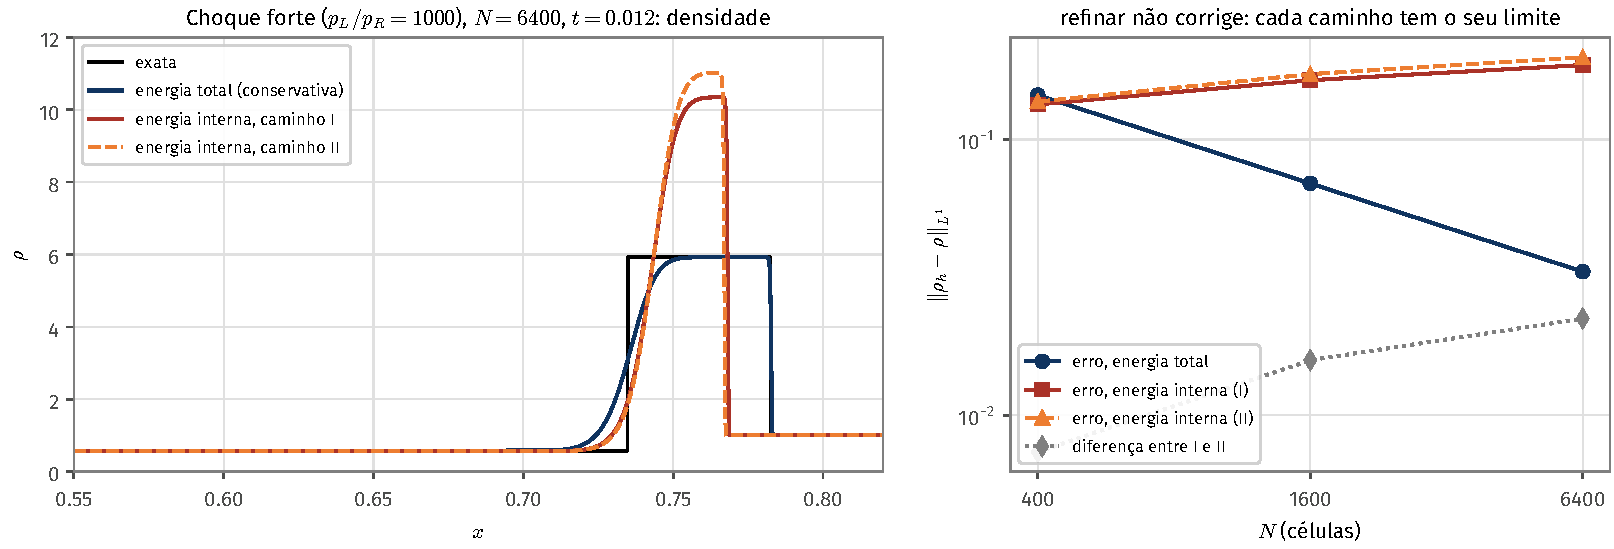
\includegraphics[width=\textwidth]{figs/energia_interna.pdf}
\caption{Euler com energia interna (forma não conservativa) contra energia total (forma conservativa). À esquerda, a densidade com $N=6400$: com a energia interna o choque anda devagar demais ($x\approx0{,}768$ em vez de $0{,}782$) e a densidade atrás dele sai perto de 10, contra $5{,}93$ na solução exata. À direita, o erro: com a energia total ele cai à metade a cada refinamento por 4; com a energia interna ele \emph{cresce}. A diferença entre os caminhos I e II também cresce: cada caminho tem o seu limite.}\label{fig:energia}
\end{figure}

A Figura~\ref{fig:energia} mostra o resultado. No tubo de Sod (razão de pressões 10) acontece o mesmo em escala menor: a diferença entre I e II fica em torno de $1{,}6\times10^{-4}$ e não diminui com a malha. O motivo é físico. O interior verdadeiro de um choque é o perfil de Navier--Stokes; ao longo dele a energia total se conserva, de modo que a conversão de energia cinética em interna tem um valor exato. Os caminhos I e II fazem essa conversão de outro modo e o estado atrás do choque sai errado. Com a energia total na forma conservativa, a conversão é contabilizada pelo fluxo e nenhum caminho é preciso.

\begin{quadro}{verde}{Regras práticas}
\begin{enumerate}[leftmargin=*]
\item Escreva na forma conservativa tudo o que puder ser conservativo (energia total, não interna).
\item Deixe os produtos não conservativos só onde a física os exige (no BN, os termos em $\partial_x\alpha$) e faça com que $\alpha$ salte apenas na onda $u_I$, linearmente degenerada.
\item Use uma discretização path-conservative; com reconstrução, o termo de volume é obrigatório (Parte~II).
\item Teste com o critério de Abgrall: com $p$ e $u$ uniformes, $p$ e $u$ devem continuar uniformes [9, 10]. Teste também contra soluções exatas de Riemann.
\item Em choques fortes que carreguem produto não conservativo, espere o erro de convergência e meça-o.
\end{enumerate}
\end{quadro}

% =====================================================================
\part*{Parte II --- A Definição 4.2 das notas de rDG do RELAP-7}
\addcontentsline{toc}{part}{Parte II --- A Definição 4.2 das notas de rDG do RELAP-7}

\section{O que a definição diz e o veredito}

As notas escrevem o modelo de sete equações como $\partial_tU+\partial_xF(U)+C(U)\,\partial_x\alpha_1=S(U)$, com $C=(u_I,0,-p_I,-p_Iu_I,0,p_I,p_Iu_I)^\top$ (equação (25) das notas). A Definição 4.2 é
\begin{equation}\label{eq:def42}
h\,\frac{\dd\ub_i}{\dd t}=-\big(\Fh_{i+1/2}-\Fh_{i-1/2}\big)-D^-_{i+1/2}-D^+_{i-1/2}-G_i+h\,\bar S_i,\qquad
G_i:=\int_{K_i}C\big(P_i(x)\big)\,\pd{P_i^\alpha}{x}\,\dd x,
\end{equation}
com $\Fh_{i+1/2}=\Fh(u_i^R,u_{i+1}^L)$, $D^-_{i+1/2}=D^-(u_i^R,u_{i+1}^L)$, $D^+_{i-1/2}=D^+(u_{i-1}^R,u_i^L)$ e $D^-+D^+=\int_\Phi C\,\dd\alpha$ ao longo do caminho do solver.

\begin{quadro}{verde}{Veredito}
\textbf{A Definição 4.2 está correta.} É o esquema de Castro, Gallardo e Parés [3] com reconstrução de estados, escrito com o fluxo conservativo separado das flutuações não conservativas. Os três termos $D^-_{i+1/2}$, $D^+_{i-1/2}$ e $G_i$ são necessários e não se sobrepõem: medem pedaços disjuntos do mesmo produto $C\,\partial_x\alpha$. Sinais, índices e argumentos estão certos. Há três acréscimos de redação recomendados (Seção~10).
\end{quadro}

\paragraph{Equivalência com Castro, Gallardo e Parés.} Em [3], para $\partial_tU+A(U)\,\partial_xU=0$ com $A(U)\,\partial_xU=\partial_xF+C\,\partial_x\alpha$, o esquema é
\[
h\,\frac{\dd\ub_i}{\dd t}=-\Big[\mathcal D^+_{i-1/2}+\mathcal D^-_{i+1/2}+\int_{K_i}A\big(P_i(x)\big)\,\pd{P_i}{x}\,\dd x\Big],
\]
com flutuações completas $\mathcal D^\pm$ (fluxo mais produto). Escrevendo $\mathcal D^-_{i+1/2}=\Fh_{i+1/2}-F(u_i^R)+D^-_{i+1/2}$, $\mathcal D^+_{i-1/2}=F(u_i^L)-\Fh_{i-1/2}+D^+_{i-1/2}$ e usando $\int_{K_i}\partial_xF(P_i)\,\dd x=F(u_i^R)-F(u_i^L)$, os termos $F(u_i^{L,R})$ cancelam e sobra exatamente~\eqref{eq:def42}. A parte conservativa interna à célula é exata (teorema fundamental do cálculo) e some na forma de fluxo; a parte não conservativa interna não tem primitiva e fica como $G_i$.

% ---------------------------------------------------------------------
\section{Por que $D^\pm$ e $G_i$ não contam a mesma coisa duas vezes}

\begin{intuicao}
Siga a solução reconstruída da esquerda para a direita, atravessando a célula $i$. Os estados percorridos formam uma corrente de três elos: o salto da face $i-\frac12$ (de $u_{i-1}^R$ a $u_i^L$), a reta dentro da célula (de $u_i^L$ a $u_i^R$) e o salto da face $i+\frac12$ (de $u_i^R$ a $u_{i+1}^L$). O produto $C\,\partial_x\alpha$ é a soma do que acontece em cada elo. $G_i$ é o elo de dentro; $D^+_{i-1/2}$ e $D^-_{i+1/2}$ são as partes dos elos de fora que cabem à célula $i$. Nenhum elo aparece duas vezes.
\end{intuicao}

\begin{figure}[h]
\centering
\begin{tikzpicture}[x=1.25cm,y=1cm,font=\small]
\draw[gray!60] (-0.3,0)--(9.3,0);
\foreach \x/\l in {0/{x_{i-3/2}},3/{x_{i-1/2}},6/{x_{i+1/2}},9/{x_{i+3/2}}}{\draw[black!35,dashed] (\x,0)--(\x,4.3); \node[below] at (\x,0) {$\l$};}
\node at (1.5,-0.55) {$K_{i-1}$}; \node at (4.5,-0.55) {$K_i$}; \node at (7.5,-0.55) {$K_{i+1}$};
\draw[azul!45,line width=1.4pt] (0,0.9)--(3,1.5);
\draw[azul,line width=2pt] (3,2.1)--(6,3.1);
\draw[azul!45,line width=1.4pt] (6,3.7)--(9,4.1);
\draw[vermelho,line width=2.2pt] (3,1.5)--(3,2.1);
\draw[vermelho,line width=2.2pt] (6,3.1)--(6,3.7);
\foreach \p in {(3,1.5),(3,2.1),(6,3.1),(6,3.7)}{\fill[black] \p circle (1.6pt);}
\node[anchor=north west] at (3.05,1.55) {$u_{i-1}^R$}; \node[anchor=north west] at (3.05,2.12) {$u_i^L$};
\node[anchor=north west] at (6.05,3.1) {$u_i^R$}; \node[anchor=south east] at (5.95,3.7) {$u_{i+1}^L$};
\node[azul,align=center,font=\footnotesize] at (4.75,1.5) {elo interior:\\ $G_i\to K_i$};
\node[vermelho,align=center,anchor=south east] at (2.9,2.0) {salto da face $i-\frac12$:\\ $D^-_{i-1/2}\to K_{i-1}$,\ \ $D^+_{i-1/2}\to K_i$};
\node[vermelho,align=center,anchor=south] at (6,4.35) {salto da face $i+\frac12$:\\ $D^-_{i+1/2}\to K_i$,\ \ $D^+_{i+1/2}\to K_{i+1}$};
\draw[decorate,decoration={brace,mirror,amplitude=6pt},laranja,thick] (3,-0.95)--(6,-0.95);
\node[laranja,below] at (4.5,-1.15) {equação de $K_i$: $\ D^+_{i-1/2}+G_i+D^-_{i+1/2}$};
\end{tikzpicture}
\caption{A corrente de estados da reconstrução $P_0P_1$ (como na Figura 5 das notas). Os saltos de face (vermelho) são repartidos pelo solver entre as duas células vizinhas; o elo interior (azul) pertence inteiro à célula. Cada elo entra uma única vez na soma sobre as células.}\label{fig:corrente}
\end{figure}

\paragraph{A conta.} Para a reconstrução afim por partes $U_h$, o produto é a medida
\[
C(U_h)\,\partial_x\alpha_h=\sum_i C(P_i)\,s_i^\alpha\,\mathbf 1_{K_i}(x)\,\dd x\;+\;\sum_{\text{faces}}\Big(\int_{\Phi(\cdot\,;\,u_i^R,\,u_{i+1}^L)}C\,\dd\alpha\Big)\,\delta_{x_{i+1/2}} .
\]
A primeira soma é a parte regular, dentro das células; a segunda é a parte singular, nas faces. A Dirac da face $x_{i+1/2}$ fica na fronteira entre $K_i$ e $K_{i+1}$ e o solver a reparte: $D^-_{i+1/2}$ para $K_i$, $D^+_{i+1/2}$ para $K_{i+1}$. Somando~\eqref{eq:def42} sobre as células,
\[
\sum_i\big(D^-_{i+1/2}+D^+_{i-1/2}+G_i\big)=\sum_{\text{faces}}\big(D^-+D^+\big)+\sum_iG_i ,
\]
que é a massa total da medida: cada pedaço aparece uma vez.

\paragraph{Por que parecem a mesma coisa.} O Lema 4.9 das notas mostra que $G_i=\int_{\Phi^{\rm seg}}C\,\dd\alpha$ ao longo do segmento de $u_i^L$ a $u_i^R$: uma integral da mesma forma que uma flutuação. São integrais da mesma natureza sobre \emph{elos diferentes}: $G_i$ liga os dois valores de face da \emph{mesma} célula; as flutuações ligam valores de face de células \emph{vizinhas}. O único objeto que representa o mesmo elo que $G_i$ é $D^-_{\rm int}+D^+_{\rm int}$ (Definição 4.10 das notas), a integral do solver entre os mesmos dois estados. Esse objeto não entra em~\eqref{eq:def42}: aparece só na análise, somado e subtraído no Lema 5.3. A diferença $E_i=G_i-(D^-_{\rm int}+D^+_{\rm int})$ registra quanto os dois caminhos discordam. A frase ``representam a mesma coisa, embora não sejam iguais'' descreve com precisão o par $\big(G_i,\ D^-_{\rm int}+D^+_{\rm int}\big)$; nenhum dos dois é contado duas vezes.

\begin{quadro}{azul}{O que a ausência de contagem dupla exige (e a Definição 4.2 cumpre)}
\begin{enumerate}[label=(\alph*),leftmargin=*]
\item \textbf{Flutuações nos valores reconstruídos} $(u_i^R,u_{i+1}^L)$, não nas médias. O salto entre médias já contém metade da variação interna de cada célula vizinha, que $G_i$ contaria de novo.
\item \textbf{Flutuações só com a parte não conservativa}, $D^-+D^+=\int_\Phi C\,\dd\alpha$. A parte conservativa inteira fica em $\Fh$; se $D^\pm$ fossem as flutuações completas, o fluxo seria contado duas vezes.
\item \textbf{$G_i$ só com a reta interior} $P_i$: integral clássica, sem escolha de caminho.
\item \textbf{$D^\pm(U,U)=0$}: sem salto, sem flutuação. Casos-limite: em $P_0$ vale $G_i=0$ e sobra o esquema de primeira ordem; numa solução suave as flutuações de face são $O(h^3)$ e sobra $G_i$ (Lema 4.3 e Observação 4.4 das notas).
\end{enumerate}
\end{quadro}

% ---------------------------------------------------------------------
\section{Verificação: o critério de Abgrall}

\begin{intuicao}
Um teste denuncia qualquer erro na combinação dos três termos: se $p$ e $u$ são uniformes nas duas fases, a interface é apenas transportada e $p$ e $u$ devem continuar uniformes. Nesse caso tudo se reduz a contar quantas vezes a variação de $\alpha$ dentro da célula entra na conta.
\end{intuicao}

\paragraph{A conta, com o fluxo de Rusanov usado no teste.} Com $p_k=p$ e $u_k=u$ uniformes, todos os estados envolvidos (médias, valores de face, pontos dos caminhos retos em variáveis conservativas, com gás rígido) têm a mesma $p$ e a mesma $u$; logo $C=C_0=(u,0,-p,-pu,0,p,pu)^\top$ é constante. Escreva $D^\pm=C_0\,d^\pm$ com $d^-+d^+=\alpha^+-\alpha^-$ em cada face (repartição central: $d^\pm=\frac12(\alpha^+-\alpha^-)$); além disso $G_i=C_0\,(\alpha_i^R-\alpha_i^L)$. O fluxo de momento da fase~1 é $F_3=u\,F_2+p\,\alpha_1$, de modo que $\Fh_3=u\,\Fh_2+p\,\bar\alpha_{i+1/2}$, com $\bar\alpha_{i+1/2}=\frac12(\alpha_i^R+\alpha_{i+1}^L)$. Em~\eqref{eq:def42},
\[
h\,\frac{\dd}{\dd t}(\alpha_1\rho_1u_1)_i-u\,h\,\frac{\dd}{\dd t}(\alpha_1\rho_1)_i
= p\,\Big[\underbrace{d^-_{i+1/2}+d^+_{i-1/2}+\big(\alpha_i^R-\alpha_i^L\big)}_{J_i}-\big(\bar\alpha_{i+1/2}-\bar\alpha_{i-1/2}\big)\Big].
\]
Com $d^-_{i+1/2}=\frac12(\alpha_{i+1}^L-\alpha_i^R)$ e $d^+_{i-1/2}=\frac12(\alpha_i^L-\alpha_{i-1}^R)$, obtém-se $J_i=\bar\alpha_{i+1/2}-\bar\alpha_{i-1/2}$ \emph{exatamente}: a velocidade não muda. O mesmo vale para a energia, logo a pressão não muda.

\begin{itemize}
\item \textbf{Sem $G_i$} (variante B), sobra $-p\,(\alpha_i^R-\alpha_i^L)=-p\,h\,s_i^\alpha$: uma força espúria proporcional à inclinação de $\alpha$. A variação interna é contada \emph{zero} vezes.
\item \textbf{Com $D^\pm$ pelas médias} (variante C), $J_i$ passa a $\frac12(\ub^\alpha_{i+1}-\ub^\alpha_{i-1})+h\,s_i^\alpha$, que excede o valor certo em $\frac h4\big(2s_i^\alpha+s_{i+1}^\alpha+s_{i-1}^\alpha\big)\approx h\,s_i^\alpha$. A variação interna é contada \emph{duas} vezes.
\item \textbf{A Definição 4.2} (variante A) conta \emph{uma} vez.
\end{itemize}
\paragraph{A mesma conta para um solver qualquer.} Suponha apenas que o solver preserva $p$ e $u$ uniformes em primeira ordem e defina $\phi_{i+1/2}:=(\Fh_3-u\,\Fh_2)_{i+1/2}/p$, com $\phi(a,a)=\alpha_a$. Aplicando essa preservação a uma célula cujos dois vizinhos são iguais a ela de um lado, obtém-se
\[
d^-(a,b)=\phi(a,b)-\alpha_a,\qquad d^+(a,b)=\alpha_b-\phi(a,b).
\]
Em~\eqref{eq:def42}, então, $J_i=\big(\phi_{i+1/2}-\alpha_i^R\big)+\big(\alpha_i^L-\phi_{i-1/2}\big)+\big(\alpha_i^R-\alpha_i^L\big)=\phi_{i+1/2}-\phi_{i-1/2}$. As flutuações trazem $-\alpha_i^R$ e $+\alpha_i^L$, os valores de face da própria célula; $G_i$ traz exatamente $\alpha_i^R-\alpha_i^L$ e a soma telescopa. É a forma mais curta de ver que $G_i$ completa as flutuações em vez de repeti-las.

\paragraph{O teste numérico.} Implementamos~\eqref{eq:def42} para o BN com gás rígido (fase 1: $\gamma=4{,}4$, $p_\infty=6\times10^8$ Pa, $\rho=1000$ kg/m$^3$; fase 2: $\gamma=1{,}4$, $\rho=1$ kg/m$^3$), fechamento $(u_I,p_I)=(u_2,p_1)$ da Definição 3.2, $p=10^5$ Pa, $u=100$ m/s, $N=200$, fluxo de Rusanov com caminho reto nas variáveis conservativas, inclinação central (Definição 4.1) com a escala de positividade (Lema 5.1), Runge--Kutta SSP de ordem 2 e CFL $0{,}1$, até 1 ms. Dois perfis de $\alpha_1$: suave ($0{,}1+0{,}8\,e^{-((x-0{,}5)/0{,}1)^2}$) e em degrau ($0{,}8$ dentro de $[0{,}25;\,0{,}75]$, $0{,}2$ fora, com densidades também em degrau).

\begin{figure}[h]
\centering
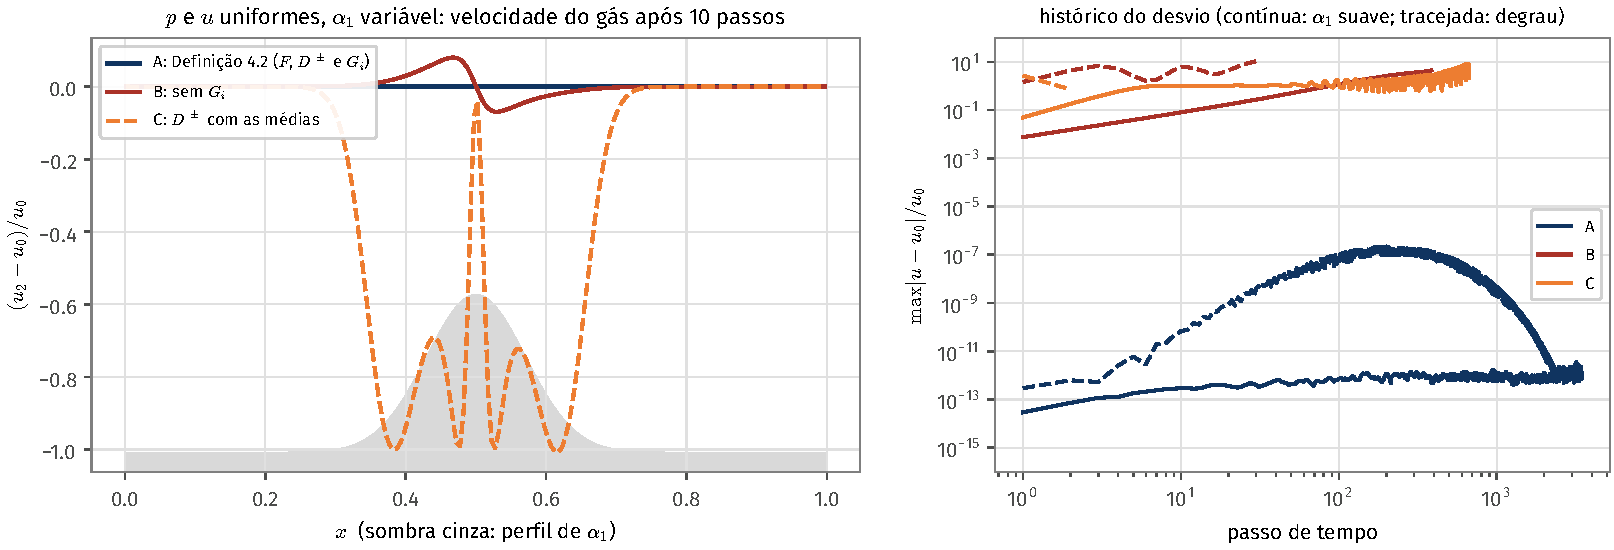
\includegraphics[width=\textwidth]{figs/def42_abgrall.pdf}
\caption{Critério de Abgrall para as três variantes. A (Definição 4.2) mantém $u$ uniforme até o arredondamento nos dois perfis. B (sem $G_i$) e C ($D^\pm$ pelas médias) criam velocidades espúrias de ordem 1 em poucos passos e terminam com estados fora do conjunto admissível.}\label{fig:abgrall}
\end{figure}

\begin{table}[h]
\centering\small
\caption{Desvio relativo máximo da velocidade, $\max|u-u_0|/u_0$.}\label{tab:abgrall}
\begin{tabular}{@{}lll@{}}
\toprule
variante & $\alpha_1$ suave & $\alpha_1$ em degrau\\
\midrule
A: Definição 4.2 & $8\times10^{-13}$ após 3450 passos & $1\times10^{-12}$ após 3453 passos\\
B: sem $G_i$ & $8\times10^{-2}$ no 10.º passo; diverge no 385.º & diverge no 31.º passo\\
C: $D^\pm$ pelas médias & $1{,}0$ no 10.º passo; diverge no 669.º & diverge no 3.º passo\\
\bottomrule
\end{tabular}
\end{table}

\begin{observacao}[Sobre o passo de tempo]
Com CFL $0{,}25$, o perfil em degrau amplificou o erro de arredondamento mesmo na variante A; com $0{,}1$ isso não ocorre. Trocando o fechamento para $(u_I,p_I)=(u_1,p_2)$, o mesmo teste roda com $0{,}25$. Trata-se da estabilidade do passo explícito neste solver de teste, não da consistência da Definição 4.2.
\end{observacao}

% ---------------------------------------------------------------------
\section{Sugestões de redação}

Nada precisa ser corrigido na Definição 4.2. Três acréscimos deixam o texto mais preciso.
\begin{enumerate}
\item Na frase que precede a definição, acrescentar $D^\pm(U,U)=0$ e a continuidade lipschitziana das flutuações. É o que faz as flutuações de face serem $O(h^3)$ em regiões suaves, passo usado no Lema 4.3 (iii).
\item Com os fechamentos de Berry (Definição 3.2), $C$ depende de $\operatorname{sgn}(\partial_x\alpha_1)$. Convém dizer que, em $G_i$, o sinal é o de $s_i^\alpha$ (constante na célula) e, na face, o do salto $\alpha^+-\alpha^-$; assim cada elo usa um único $C$.
\item No pseudocódigo da Seção 5.3 (passo 4), escrever explicitamente que $P_i$ é a reta já escalada, $\ub_i+\theta_is_i\xi$. Assim $G_i$ liga exatamente os valores de face usados no passo 3 e a corrente de estados não se rompe.
\end{enumerate}

% ---------------------------------------------------------------------
\section*{Referências}
\addcontentsline{toc}{section}{Referências}
\small
\begin{enumerate}[label={[\arabic*]},leftmargin=*]
\item G. Dal Maso, P. G. LeFloch, F. Murat. Definition and weak stability of nonconservative products. \emph{J. Math. Pures Appl.} 74 (1995) 483--548.
\item C. Parés. Numerical methods for nonconservative hyperbolic systems: a theoretical framework. \emph{SIAM J. Numer. Anal.} 44 (2006) 300--321.
\item M. J. Castro, J. M. Gallardo, C. Parés. High order finite volume schemes based on reconstruction of states for solving hyperbolic systems with nonconservative products. Applications to shallow-water systems. \emph{Math. Comp.} 75 (2006) 1103--1134.
\item M. J. Castro, P. G. LeFloch, M. L. Muñoz-Ruiz, C. Parés. Why many theories of shock waves are necessary: convergence error in formally path-consistent schemes. \emph{J. Comput. Phys.} 227 (2008) 8107--8129.
\item R. Abgrall, S. Karni. A comment on the computation of non-conservative products. \emph{J. Comput. Phys.} 229 (2010) 2759--2763.
\item T. Y. Hou, P. G. LeFloch. Why nonconservative schemes converge to wrong solutions: error analysis. \emph{Math. Comp.} 62 (1994) 497--530.
\item N. Andrianov, G. Warnecke. The Riemann problem for the Baer--Nunziato two-phase flow model. \emph{J. Comput. Phys.} 195 (2004) 434--464.
\item D. W. Schwendeman, C. W. Wahle, A. K. Kapila. The Riemann problem and a high-resolution Godunov method for a model of compressible two-phase flow. \emph{J. Comput. Phys.} 212 (2006) 490--526.
\item R. Abgrall. How to prevent pressure oscillations in multicomponent flow calculations: a quasi conservative approach. \emph{J. Comput. Phys.} 125 (1996) 150--160.
\item R. Saurel, R. Abgrall. A multiphase Godunov method for compressible multifluid and multiphase flows. \emph{J. Comput. Phys.} 150 (1999) 425--467.
\item RELAP5/MOD3.3 Code Manual, Vol.\ I: Code Structure, System Models, and Solution Methods. NUREG/CR-5535/Rev 1, 2001.
\end{enumerate}

\end{document}
